% Options for packages loaded elsewhere
% Options for packages loaded elsewhere
\PassOptionsToPackage{unicode}{hyperref}
\PassOptionsToPackage{hyphens}{url}
\PassOptionsToPackage{dvipsnames,svgnames,x11names}{xcolor}
%
\documentclass[
  11pt,
  a4paper,
]{article}
\usepackage{xcolor}
\usepackage{amsmath,amssymb}
\setcounter{secnumdepth}{-\maxdimen} % remove section numbering
\usepackage{iftex}
\ifPDFTeX
  \usepackage[T1]{fontenc}
  \usepackage[utf8]{inputenc}
  \usepackage{textcomp} % provide euro and other symbols
\else % if luatex or xetex
  \usepackage{unicode-math} % this also loads fontspec
  \defaultfontfeatures{Scale=MatchLowercase}
  \defaultfontfeatures[\rmfamily]{Ligatures=TeX,Scale=1}
\fi
\usepackage{lmodern}
\ifPDFTeX\else
  % xetex/luatex font selection
\fi
% Use upquote if available, for straight quotes in verbatim environments
\IfFileExists{upquote.sty}{\usepackage{upquote}}{}
\IfFileExists{microtype.sty}{% use microtype if available
  \usepackage[]{microtype}
  \UseMicrotypeSet[protrusion]{basicmath} % disable protrusion for tt fonts
}{}
\usepackage{setspace}
\makeatletter
\@ifundefined{KOMAClassName}{% if non-KOMA class
  \IfFileExists{parskip.sty}{%
    \usepackage{parskip}
  }{% else
    \setlength{\parindent}{0pt}
    \setlength{\parskip}{6pt plus 2pt minus 1pt}}
}{% if KOMA class
  \KOMAoptions{parskip=half}}
\makeatother
% Make \paragraph and \subparagraph free-standing
\makeatletter
\ifx\paragraph\undefined\else
  \let\oldparagraph\paragraph
  \renewcommand{\paragraph}{
    \@ifstar
      \xxxParagraphStar
      \xxxParagraphNoStar
  }
  \newcommand{\xxxParagraphStar}[1]{\oldparagraph*{#1}\mbox{}}
  \newcommand{\xxxParagraphNoStar}[1]{\oldparagraph{#1}\mbox{}}
\fi
\ifx\subparagraph\undefined\else
  \let\oldsubparagraph\subparagraph
  \renewcommand{\subparagraph}{
    \@ifstar
      \xxxSubParagraphStar
      \xxxSubParagraphNoStar
  }
  \newcommand{\xxxSubParagraphStar}[1]{\oldsubparagraph*{#1}\mbox{}}
  \newcommand{\xxxSubParagraphNoStar}[1]{\oldsubparagraph{#1}\mbox{}}
\fi
\makeatother


\usepackage{longtable,booktabs,array}
\newcounter{none} % for unnumbered tables
\usepackage{calc} % for calculating minipage widths
% Correct order of tables after \paragraph or \subparagraph
\usepackage{etoolbox}
\makeatletter
\patchcmd\longtable{\par}{\if@noskipsec\mbox{}\fi\par}{}{}
\makeatother
% Allow footnotes in longtable head/foot
\IfFileExists{footnotehyper.sty}{\usepackage{footnotehyper}}{\usepackage{footnote}}
\makesavenoteenv{longtable}
\usepackage{graphicx}
\makeatletter
\newsavebox\pandoc@box
\newcommand*\pandocbounded[1]{% scales image to fit in text height/width
  \sbox\pandoc@box{#1}%
  \Gscale@div\@tempa{\textheight}{\dimexpr\ht\pandoc@box+\dp\pandoc@box\relax}%
  \Gscale@div\@tempb{\linewidth}{\wd\pandoc@box}%
  \ifdim\@tempb\p@<\@tempa\p@\let\@tempa\@tempb\fi% select the smaller of both
  \ifdim\@tempa\p@<\p@\scalebox{\@tempa}{\usebox\pandoc@box}%
  \else\usebox{\pandoc@box}%
  \fi%
}
% Set default figure placement to htbp
\def\fps@figure{htbp}
\makeatother





\setlength{\emergencystretch}{3em} % prevent overfull lines

\providecommand{\tightlist}{%
  \setlength{\itemsep}{0pt}\setlength{\parskip}{0pt}}



 


\makeatletter
\@ifpackageloaded{caption}{}{\usepackage{caption}}
\AtBeginDocument{%
\ifdefined\contentsname
  \renewcommand*\contentsname{Table of contents}
\else
  \newcommand\contentsname{Table of contents}
\fi
\ifdefined\listfigurename
  \renewcommand*\listfigurename{List of Figures}
\else
  \newcommand\listfigurename{List of Figures}
\fi
\ifdefined\listtablename
  \renewcommand*\listtablename{List of Tables}
\else
  \newcommand\listtablename{List of Tables}
\fi
\ifdefined\figurename
  \renewcommand*\figurename{Figure}
\else
  \newcommand\figurename{Figure}
\fi
\ifdefined\tablename
  \renewcommand*\tablename{Table}
\else
  \newcommand\tablename{Table}
\fi
}
\@ifpackageloaded{float}{}{\usepackage{float}}
\floatstyle{ruled}
\@ifundefined{c@chapter}{\newfloat{codelisting}{h}{lop}}{\newfloat{codelisting}{h}{lop}[chapter]}
\floatname{codelisting}{Listing}
\newcommand*\listoflistings{\listof{codelisting}{List of Listings}}
\makeatother
\makeatletter
\makeatother
\makeatletter
\@ifpackageloaded{caption}{}{\usepackage{caption}}
\@ifpackageloaded{subcaption}{}{\usepackage{subcaption}}
\makeatother
\usepackage{bookmark}
\IfFileExists{xurl.sty}{\usepackage{xurl}}{} % add URL line breaks if available
\urlstyle{same}
\hypersetup{
  pdftitle={RENTASALUD: a web-based interactive atlas of social inequalities and life expectancy in Andalusia (southern Spain)},
  colorlinks=true,
  linkcolor={blue},
  filecolor={Maroon},
  citecolor={Blue},
  urlcolor={Blue},
  pdfcreator={LaTeX via pandoc}}


\title{RENTASALUD: a web-based interactive atlas of social inequalities
and life expectancy in Andalusia (southern Spain)}
\author{Gustavo Rivas Gervilla \and Paloma Massó Guijarro \and Maja
Nikšić \and Mario Rivera Izquierdo \and Miguel Ángel
Montero-Alonso \and Juan Manuel Melchor Rodríguez \and Miguel Ángel
Luque-Fernández}
\date{2026-08-06}
\begin{document}
\maketitle
\begin{abstract}
\textbf{Background} Interactive tools linking income and life expectancy
at fine geographical scales are scarce for southern Europe.
\textbf{Methods} We linked INE census-section income data (48,262
section-years, 2015--2022) with BDLPA cohort life tables
(\textasciitilde637,000 individuals, follow-up 2011--2023) for
Andalusia, Ceuta, and Melilla. \textbf{Results} Life expectancy was 79.5
(men) and 84.4 years (women). Tumours yielded the largest potential gain
for men (3.93 years) and heart disease for women (2.89 years). The
provincial income--LE correlation was weak (r=0.28, P=0.43), rising to
r=0.52 with Ceuta and Melilla excluded. Provincial LE ranged from 79.4
(Almería) to 82.7 years (Córdoba). \textbf{Conclusion} Provincial
aggregation attenuates the income--life expectancy gradient;
neighbourhood-level tools like RENTASALUD are needed to detect
inequalities. \textbf{Keywords:} health inequalities, life expectancy,
spatial epidemiology, interactive atlas, Andalusia ~GRG and PMG
contributed equally as co-first authors.
\end{abstract}


\setstretch{1.5}
\section{What is already known on this
topic}\label{what-is-already-known-on-this-topic}

\begin{itemize}
\tightlist
\item
  People in Spain's most deprived neighbourhoods live 3--4 years less
  than those in the wealthiest.
\item
  Southern Europe has smaller health inequalities than Northern or
  Eastern Europe.
\item
  Interactive tools linking neighbourhood income and life expectancy are
  rare.
\end{itemize}

\section{What this study adds}\label{what-this-study-adds}

\begin{itemize}
\tightlist
\item
  RENTASALUD is an open source interactive atlas of census-section
  income and life expectancy for Andalusia, Ceuta, and Melilla.
\item
  At province level the income--LE correlation is weak (r=0.28) and
  doubles when income-outlier cities are excluded (r=0.52).
\item
  Cancer and cardiovascular disease account for 7.1 years of potential
  LE gain in men and 5.7 in women.
\item
  A built-in AI assistant lets anyone query the data in plain language.
\end{itemize}

\section{Introduction}\label{introduction}

In Spain, people living in the most deprived neighbourhoods die 3 to 4
years earlier than those in the wealthiest {[}@redondo2022{]}. The
gradient is steep, and it varies by region. Andalusia, Spain's largest
and one of its poorest regions, is home to some 8.5 million people. Yet
few interactive tools allow researchers, policymakers, or the public to
explore how income and life expectancy relate at the neighbourhood
scale. Most available maps cover entire provinces, losing the
within-area variation that drives the gradient.

RENTASALUD was built to fill that gap: a free, open source web atlas
that combines detailed census-section data (INE, 2015--2022) with cohort
life tables from the Longitudinal Database of the Andalusian Population
(BDLPA, \textasciitilde637,000 individuals followed from the 2011 census
through 2023). The analysis covers the eight Andalusian provinces plus
the autonomous cities of Ceuta and Melilla. We estimated life expectancy
(LE) by province, sex, and cause of death, examined the
income--longevity association, and deployed everything as an interactive
Shiny application with an AI-powered natural-language interface.

\section{Methods}\label{methods}

Income and demographic data come from the INE \emph{Atlas de
Distribución de Renta de los Hogares} {[}@ine\_adrh\_metodologia{]},
providing 48,262 census-section observations (2015--2022) across ten
territories. Mortality data come from the BDLPA
{[}@ieca\_bdlpa\_metodologia{]}, a 10\% random sample of the 2011
Andalusian census with follow-up through December 2023. Causes of death
were grouped into ten broad categories.

We used standard abridged life table methods {[}@chiang1968{]} with
5-year age bands (0--4 through 85--89, 90+) to estimate life expectancy
at birth by sex. Cause-deleted life tables {[}@beltran-sanchez2008{]}
quantified potential gains from eliminating each cause, using Chiang's
proportional-risk adjustment. Twenty life tables were constructed (10
territories × 2 sexes). Census-tract estimation was not feasible because
BDLPA identifiers carry no sub-provincial geographic code.

We examined the province-level association between mean income and life
expectancy using Pearson and Spearman correlations. As a sensitivity
check we repeated the analysis excluding Ceuta and Melilla, two
autonomous cities whose economies rely on cross-border trade and
public-sector employment, making them structurally different from the
Andalusian provinces. The study was approved by the University of
Granada Ethics Committee (SOCESVIDA, SICEIA-2025-000814).

\section{Results}\label{results}

Life expectancy at birth was 79.5 years for men and 84.4 for women, a
gap of nearly 5 years. Provincial LE ranged from 77.8 years (Almería,
men) to 80.1 (Córdoba and Cádiz, men) and from 80.9 (Almería, women) to
85.3 (Córdoba, women). The mean provincial spread was 3.3 years (79.4 in
Almería to 82.7 in Córdoba).

Eliminating malignant tumours would add 3.93 years to male life
expectancy at birth and 2.83 to female (Table 1). For women, heart and
circulatory disease had the largest impact (2.89 years). Together,
tumours and cardiovascular disease accounted for 7.1 years of potential
gain in men and 5.7 in women. Men lost 1.1 more years to cancer than
women, consistent with historically higher smoking rates in Spanish men.

\begin{longtable}[]{@{}lll@{}}
\caption{Years gained at birth if each cause were
eliminated.}\tabularnewline
\toprule\noalign{}
Cause & Men (years) & Women (years) \\
\midrule\noalign{}
\endfirsthead
\toprule\noalign{}
Cause & Men (years) & Women (years) \\
\midrule\noalign{}
\endhead
\bottomrule\noalign{}
\endlastfoot
Malignant tumours & 3.93 & 2.83 \\
Heart and circulatory diseases & 3.15 & 2.89 \\
Respiratory diseases & 1.13 & 0.69 \\
External causes (accidents, suicide) & 0.67 & 0.33 \\
Digestive diseases & 0.57 & 0.48 \\
Nervous system diseases & 0.50 & 0.57 \\
Infectious diseases & 0.41 & 0.35 \\
Diabetes and endocrine diseases & 0.28 & 0.32 \\
Alcohol-related causes & 0.07 & 0.02 \\
Other causes & 1.13 & 1.19 \\
\end{longtable}

Province-level income and life expectancy were weakly correlated
(r=0.28, 95\% CI −0.42 to 0.77, P=0.43; Spearman ρ=0.24, P=0.51). Ceuta
(€16,899, LE 82.2) and Melilla (€15,443, LE 82.4) are income outliers:
their median incomes are well above the Andalusian range
(€12,699--€14,338), but their life expectancy sits in the middle,
weakening the aggregate association. Excluding them raises the
correlation to r=0.52 (P=0.19, R²=0.29).

\begin{figure}

\centering{

\pandocbounded{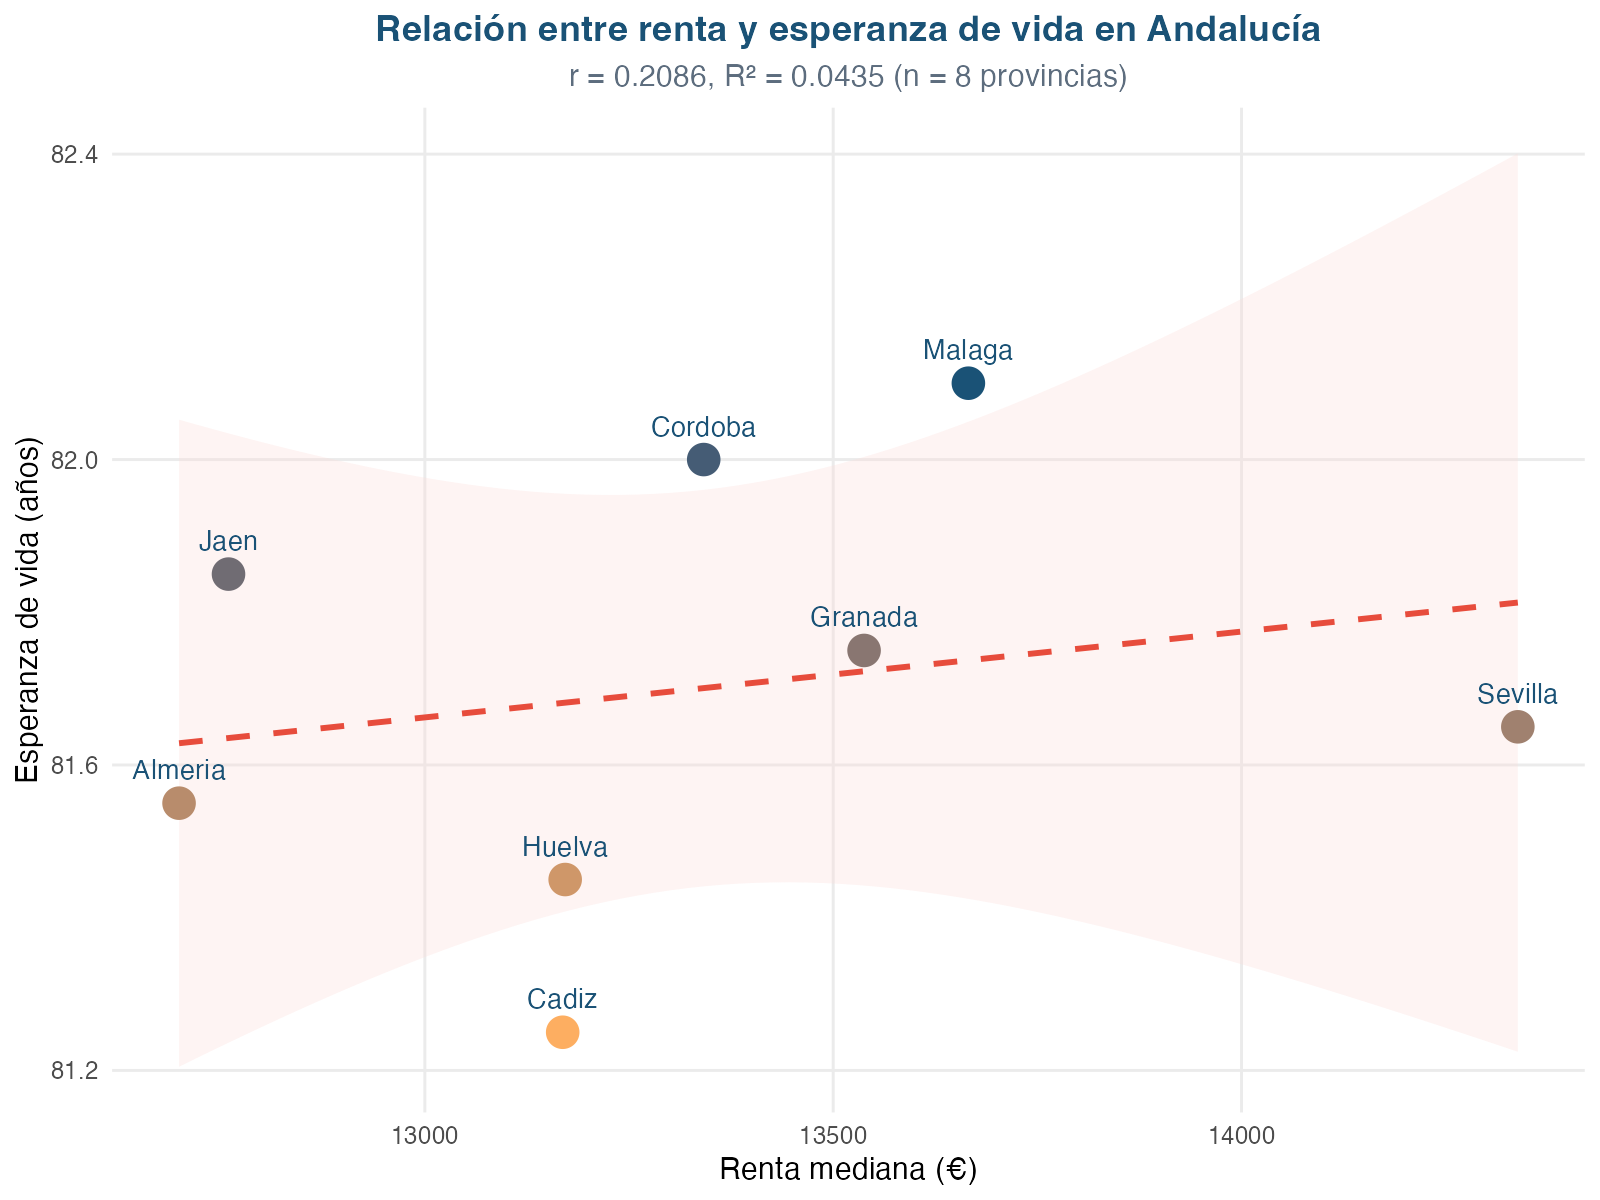
\includegraphics[keepaspectratio]{figures/renta_vs_ev_scatter.png}}

}

\caption{\label{fig-scatter}Income vs life expectancy across provinces.
Blue: Andalusian provinces. Red: Ceuta and Melilla (income outliers).
Solid line: fit without Ceuta/Melilla (R²=0.29, P=0.17). Dashed line:
all ten territories (R²=0.08, P=0.43).}

\end{figure}%

The 3.3-year provincial gradient runs in the expected direction, but the
statistical signal is imprecise with ten data points. Redondo-Sánchez et
al.~found a much steeper gradient at census-tract level (3.8 years for
men, 3.2 for women) {[}@redondo2022{]}, suggesting that within-province
disparities likely exceed what we can detect here. The results are
available through an interactive R Shiny application at
\href{https://watzile.shinyapps.io/RENTA/}{watzile.shinyapps.io/RENTA}
with all analysis code at
\href{https://github.com/migariane/RENTASALUD}{github.com/migariane/RENTASALUD}.

\section{Discussion}\label{discussion}

The province-level income--LE correlation is weak mainly for two
reasons: aggregating thousands of census tracts into ten units shrinks
variance, and Ceuta and Melilla act as leverage points with high incomes
but mid-range life expectancy. Removing them triples the explained
variance. The 3.3-year provincial spread in life expectancy is real, but
its statistical expression is noisy at n=10.

This study links individual follow-up on nearly 637,000 people over 12
years to fine-grained socioeconomic data. The main limitation is
geographic: BDLPA person identifiers contain no sub-provincial code,
restricting LE estimation to the province level. Future linkage to the
municipal register (Padrón Continuo) would enable small-area Bayesian
estimation. Other limitations include constant-mortality assumptions,
small cell counts at extreme ages, and the standard caveat that
cause-deleted life tables treat causes as independent.

\section{Acknowledgements}\label{acknowledgements}

Supported by the Plan Propio de Investigacion y Transferencia,
University of Granada (2025, Programa 21). BDLPA data provided by the
IECA.

\section{Data Availability}\label{data-availability}

Analysis code:
\href{https://github.com/migariane/RENTASALUD}{github.com/migariane/RENTASALUD}.
Shiny application:
\href{https://watzile.shinyapps.io/RENTA/}{watzile.shinyapps.io/RENTA}.
BDLPA microdata available from IECA on request.

\section{References}\label{references}

\begin{enumerate}
\def\labelenumi{\arabic{enumi}.}
\item
  Redondo-Sánchez D, Sánchez MJ, Fernández-Navarro P, Rachet B,
  Luque-Fernandez MA. Association of socioeconomic deprivation with life
  expectancy and all-cause mortality in Spain, 2011-2013. \emph{Sci
  Rep}. 2022;12(1):15554. doi:10.1038/s41598-022-19859-1.
\item
  Marmot M. \emph{Fair Society, Healthy Lives: The Marmot Review}.
  London: UCL; 2010.
\item
  Mackenbach JP, Kulhánová I, Menvielle G, et al.~Trends in inequalities
  in premature mortality: a study of 3.2 million deaths in 13 European
  countries. \emph{J Epidemiol Community Health}. 2015;69(3):207-17.
  doi:10.1136/jech-2014-204319.
\item
  Mackenbach JP, Valverde JR, Artnik B, et al.~Trends in health
  inequalities in 27 European countries. \emph{Proc Natl Acad Sci}.
  2018;115(25):6440-5. doi:10.1073/pnas.1800028115.
\item
  Regidor E, Kunst AE, Rodríguez-Artalejo F, Mackenbach JP. Small
  socio-economic differences in mortality in Spanish older people.
  \emph{Eur J Public Health}. 2012;22(1):80-5.
  doi:10.1093/eurpub/ckr051.
\item
  Regidor E, Reques L, Belza MJ, et al.~Education and mortality in
  Spain: a review of the literature. \emph{Gac Sanit}. 2014;28(6):492-8.
  doi:10.1016/j.gaceta.2014.06.001.
\item
  Chiang CL. \emph{Introduction to Stochastic Processes in
  Biostatistics}. New York: Wiley; 1968.
\item
  Beltrán-Sánchez H, Preston SH, Canudas-Romo V. An integrated approach
  to cause-of-death analysis: cause-deleted life tables and
  decompositions of life expectancy. \emph{Demogr Res}.
  2008;19:1565-602. doi:10.4054/DemRes.2008.19.35.
\item
  Instituto Nacional de Estadística. Atlas de Distribución de Renta de
  los Hogares: Metodología. 2024.
  https://www.ine.es/dyngs/INEbase/es/operacion.htm?c=Estadistica\_C\&cid=1254736177088\&menu=metodologia.
\item
  Instituto de Estadística y Cartografía de Andalucía. Estadísticas
  Longitudinales de Supervivencia y Longevidad en Andalucía: Ficheros de
  Microdatos, Cohorte 2011. 2024.
  https://www.juntadeandalucia.es/institutodeestadisticaycartografia/bdlpa/.
\end{enumerate}




\end{document}
